\subsection{Model Architecture}
\label{sec:arch}

\begin{figure}[!t]
\centering
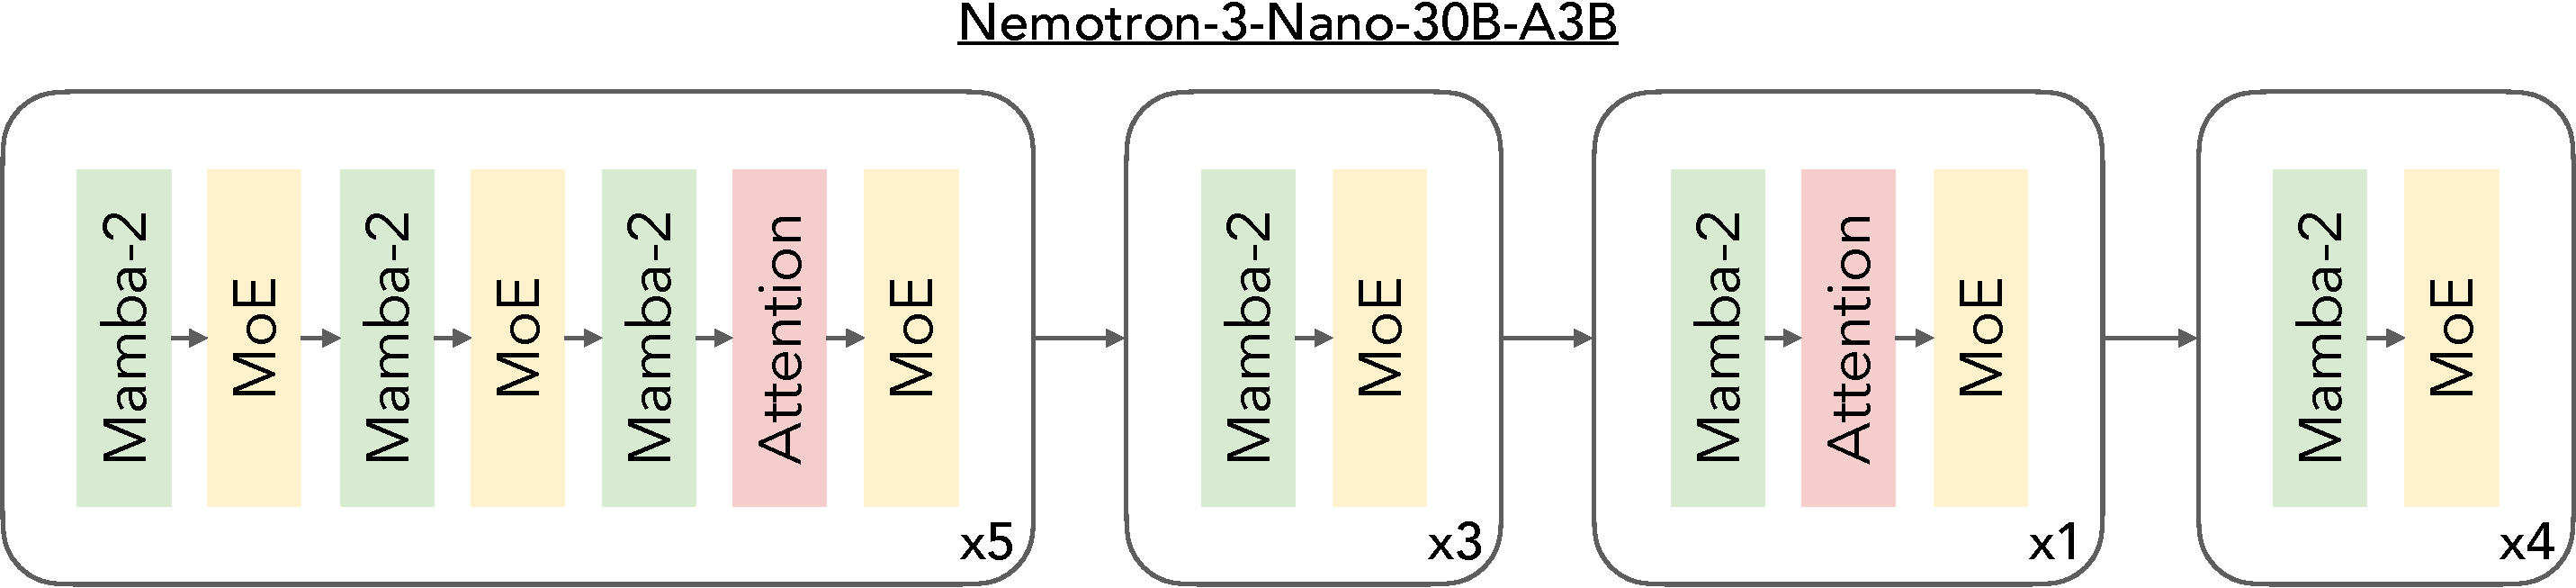
\includegraphics[width=0.9\linewidth]{figures/pattern.pdf}
\caption{\ourmodel layer pattern. We use a hybrid Mamba-Transformer architecture similar to the previous generation of Nemotron models. In addition, we scale the model sparsely by using MoE layers instead of standard FFN layers.}
\label{fig:layer-pattern}
\end{figure}

\begin{table*}[!hbt]\small\centering
\renewcommand{\arraystretch}{1.2} % adjust row height for readability
\setlength{\tabcolsep}{6pt} % adjust column padding
\begin{tabular}{l|c}
\toprule
\textbf{Model} & \textbf{\ourbasemodel} \\
\midrule
Num Layers         & 52  \\
Model Dimension             & 2688 \\
\midrule
Q-heads             & 32 \\
KV-heads             & 2 \\
Head Dimension             & 128 \\
\midrule
Mamba State Dimension             & 128 \\
Mamba Groups             & 8 \\
Mamba Heads         & 64 \\
Mamba Head Dimension      & 64 \\
\midrule
Expert Dimension           & 1856 \\
Total Routable Experts             & 128 \\
Number of Activated Experts             & 6 \\
Number of Shared Experts             & 2 \\

\bottomrule
\end{tabular}
\caption{\ourmodel Architecture}
\label{table:model_arch}
\end{table*}

\ourbasemodel builds upon the hybrid Mamba-Transformer architecture of our older Nemotron-H~\citep{nvidia2025nemotronhfamilyaccurateefficient} and Nemotron 2 Nano~\citep{nemotronnanov2} models by replacing the standard FFN layers with sparse Mixture-of-Experts (MoE)~\citep{shazeer2017outrageously} layers. The MoE layers help us achieve better accuracy at a fraction of the active parameter count. \ourbasemodel contains 31.6B total parameters out of which 3.2B are active (3.6B including embeddings) per forward pass. To achieve the best accuracy, we use a granular MoE architecture along with shared experts~\citep{dai2024deepseekmoe}. For the MoE layers, we use squared ReLU activation and a standard learnt MLP router with sigmoid gating. We do not use any positional embeddings, dropout, or bias on linear layers. We use RMSNorm for normalization and un-tie embedding and projection weights.
% We enlist the key architectural components for \ourmodel below:

% \newparagraph{Grouped-Query-Attention:} We use 6 GQA layers with 32 Query-heads, 2 KV-heads, and 128 per-head-dimension.  

% \newparagraph{Mamba:} We use 23 Mamba layers with 64 heads and a head-dim of 64. 

% \newparagraph{Mixture-of-Experts:} We use 128 granular experts~\citep{} each with a dimension of 1856   

Table~\ref{table:model_arch} and Figure~\ref{fig:layer-pattern} show the key architectural details of \ourmodel.